%======================================================================
% 5. RESULTS: DETERMINISTIC VS ROBUST FRONTS
%======================================================================
\section{Results: deterministic vs robust fronts}
\label{sec:results}

The deterministic front was generated on the surrogate at $\mathbf{z}_0$ and
then re-evaluated through the moment engine; the robust front is native to
it. Unless stated otherwise, every number in this section is a
common-random-number moment at $n_z=2000$ with the inflated $\sigma$ of
Eq.~\eqref{eq:infl}. Both final populations are feasible in their own
formulation and, at reporting precision, non-dominated.

\subsection{Front geometry and the dispersion floor}
\label{sec:fronts}

Figure~\ref{fig:front} places both fronts in the
$\mathrm{E}[Q_s]$--$\sigma_{Q_s}$ plane. Two features organize everything
that follows. The first is the dispersion floor: the minimum attainable
$\sigma_{Q_s}$ is \SI{16.4}{\mega\joule\per\square\metre} (coefficient of
variation 19.9\%), and it is the same for both fronts --- a property of
the uncertainty model, principally the $\gamma_0$ dispersion, that no
shape in the studied three-parameter space reaches below. The floor is
geometry-insensitive \emph{within this design space and uncertainty
model}; Section~\ref{sec:sens} shows how it scales when the assumed
dispersions change, and we make no claim of a universal physical bound. The second is where the fronts sit relative
to that floor: the robust front tracks it closely over its whole length,
while the deterministic front, optimized without any dispersion term,
wanders up to three times higher in $\sigma_{Q_s}$ at comparable expected
heat load. The projections of Fig.~\ref{fig:projections} show the same
structure in the performance objectives: the fronts overlap substantially
in $(\eta_V,\mathrm{E}[Q_s])$ and $(\mathrm{E}[sg],\mathrm{E}[Q_s])$, so
robustness is not bought with a separate region of the performance space
but with different designs at like performance.

\begin{figure}[htbp]
\centering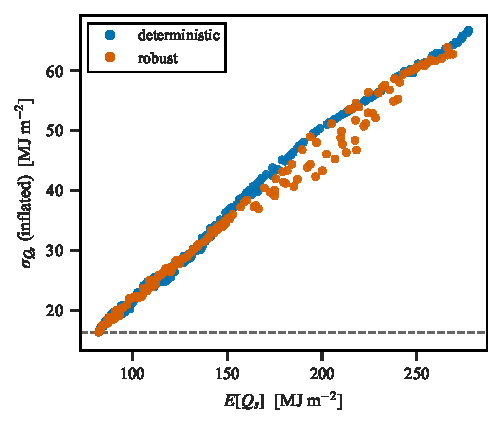
\includegraphics[width=\linewidth]{fig1_front_sigma}
\caption{Deterministic (blue) and robust (vermillion) fronts in the
  $\mathrm{E}[Q_s]$--$\sigma_{Q_s}$ plane (common-random-number moments,
  $n_z=2000$, inflated $\sigma$). Dashed: geometry-insensitive dispersion
  floor $\sigma_{Q_s}=\SI{16.4}{\mega\joule\per\square\metre}$ (CV
  19.9\%), identical on both fronts -- set by the $\gamma_0$ dispersion,
  not by shape.}
\label{fig:front}
\end{figure}
\begin{figure}[htbp]
\centering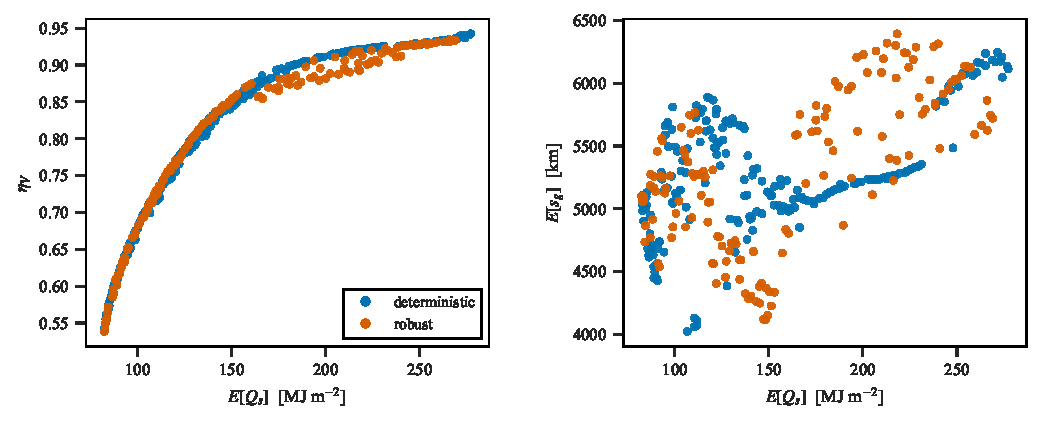
\includegraphics[width=\linewidth]{fig4_front_projections}
\caption{Front projections: volumetric efficiency $\eta_V$ and expected
  range $\mathrm{E}[sg]$ versus $\mathrm{E}[Q_s]$.}
\label{fig:projections}
\end{figure}

\subsection{Matched-performance comparison}
\label{sec:matched}

Front medians are not comparable across a three- against four-objective
formulation, so the comparison is made design against design. A
deterministic design and a robust design form a \emph{matched pair} when
the robust design matches expected heat load and range within a narrow
window ($\mathrm{E}[Q_s]$ at most 2\% higher, $\mathrm{E}[sg]$ at most 2\%
lower); the quantity of interest is then the $\sigma_{Q_s}$ reduction the
robust design achieves at that performance. Of the 200 deterministic
designs, 196 have at least one robust match --- a median of 26 eligible
partners each --- yielding 5{,}371 pairs. In 98.1\% of those pairs the
robust design has the lower $\sigma_{Q_s}$, and the median cut at pair
level is 27.5\% (quartiles 14--47\%; Table~\ref{tab:matched}). These are
descriptive statistics of the constructed comparison set: the 5{,}371
pairs share 196 deterministic and 150 robust designs, so they are not
independent trials, and no sampling interval is attached to them; their
stability across optimizer seeds is reported separately
(Appendix~\ref{app:seeds}).

Because a deterministic design typically has many eligible partners, any
design-level summary depends on the partner-selection rule, and we report
two bounds of it (Table~\ref{tab:matched}, Fig.~\ref{fig:matched}).
Selecting the eligible partner with the lowest $\sigma_{Q_s}$ --- the
envelope of the robust front at matched performance, and the design an
engineer would actually adopt --- improves 99.5\% of the 196 designs,
with a median cut of 35.0\%. This selection examines the outcome, so it
is complemented by a prespecified rule that cannot: the eligible partner
\emph{nearest in relative performance space} (Euclidean distance in the
two matching ratios, ties broken by front index). Under that rule 84.2\%
of designs are still improved, with a median cut of 4.3\%. The gap
between the two rules is structural, not statistical: at matched
performance the robust front offers a spread of $\sigma_{Q_s}$ --- a
median factor 1.49 between the extreme eligible partners --- because
$\sigma_{Q_s}$ is itself an objective traded against $\eta_V$. The
nearest performance neighbour is typically a member of that spread whose
$\sigma_{Q_s}$ resembles the deterministic design's own --- in the
low-load tercile the chosen partners sit at the 11th
$\sigma$-percentile of the robust front (both fronts sit on the floor
there), in the high-load tercile at the 81st (the robust front's own
high-$\sigma$ extreme members) --- while the envelope is the lower edge
of the same spread. Both rules locate the advantage in the same place:
the envelope cut grows monotonically across heat-load terciles of the
deterministic front (14.6\%, 45.8\%, 63.7\%), while the
nearest-neighbour cut peaks in the middle tercile (1.5\%, 14.5\%,
2.2\%). Restricting the window to bind in both legs (both ratios
within $\pm$2\%; 136 of the 5{,}371 pairs) collapses the median cut to
0.4\%: the advantage is carried by the one-sided slack the window
allows --- robust designs delivering less expected heat load at no less
range --- rather than by equal-performance designs differing in
$\sigma_{Q_s}$ alone. The worst members also improve: the maximum exceedance
probabilities over each front roughly halve under the robust formulation
(Table~\ref{tab:matched}, lower rows).

\begin{figure}[htbp]
\centering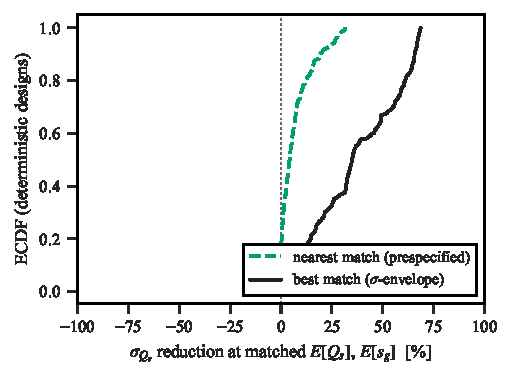
\includegraphics[width=\linewidth]{fig2_matched_sigma_cut}
\caption{ECDF over deterministic designs of the $\sigma_{Q_s}$ reduction
  at matched performance (window $\mathrm{E}[Q_s]+2\%$,
  $\mathrm{E}[sg]-2\%$) under two partner-selection rules: the
  prespecified nearest-performance match (green dashed) and the
  lowest-$\sigma$ eligible partner, i.e.\ the robust front's
  $\sigma$-envelope at matched performance (black). Median cuts 4.3\%
  and 35.0\%; 196/200 designs matched; 98.1\% of the 5{,}371 matched
  pairs favour the robust front.}
\label{fig:matched}
\end{figure}
\begin{table}[htbp]
\centering
\caption{Matched-performance comparison of the fronts (window
  $\mathrm{E}[Q_s]+2\%$, $\mathrm{E}[sg]-2\%$, inflated $\sigma$).}
\label{tab:matched}
\begin{tabular}{lc}
\toprule
statistic & value \\
\midrule
deterministic designs with $\geq$1 robust match & 196 / 200 \\
matched (det, robust) pairs & 5{,}371 \\
pairs with $\sigma_{\mathrm{rob}}<\sigma_{\mathrm{det}}$ & 98.1\% \\
pair-level median $\sigma_{Q_s}$ cut & 27.5\% \\
design-level: designs improved by best match ($\sigma$-envelope) &
  99.5\% \\
design-level median best-match cut (Fig.~\ref{fig:matched}) & 35.0\% \\
design-level: designs improved by nearest match (prespecified) &
  84.2\% \\
design-level median nearest-match cut (Fig.~\ref{fig:matched}) &
  4.3\% \\
median $\sigma$-spread of eligible partners (max/min) & 1.49 \\
worst-member $P(q_{\mathrm{stag}}>\mathrm{lim})$, det / robust &
  6.8\% / 4.8\% \\
worst-member $P(q_{\mathrm{shldr}}>\mathrm{lim})$, det / robust &
  10.0\% / 6.6\% \\
\bottomrule
\end{tabular}
\end{table}

\subsection{The hidden cost of deterministic design}
\label{sec:audit}

The deterministic front satisfies every constraint of Eq.~\eqref{eq:detcon}
at $\mathbf{z}_0$ exactly. Under the uncertainty model, however, a
point-feasible design is a distribution, and the deterministic formulation
never looks at that distribution. The post-hoc audit
(Table~\ref{tab:audit}, Fig.~\ref{fig:violation}) quantifies what is
concealed. The median $\sigma_{Q_s}$ hidden on the deterministic front is
\SI{30.3}{\mega\joule\per\square\metre} (median coefficient of variation
22.8\%). One in four deterministic designs carries a stagnation-heating
exceedance probability above 1\% (maximum 6.8\%), and nearly one in four a
shoulder-heating exceedance probability above 1\% (maximum 10.0\%); the
load-factor constraint is never active under dispersion. Requiring
robust-style feasibility ($\mathrm{E}+2\sigma$) would remove 8\% of the
deterministic front. None of this is visible from the deterministic
problem's own outputs, which report all constraints as satisfied ---
Section~\ref{sec:verification} confirms the largest of these probabilities
against the true simulator.

\begin{figure}[htbp]
\centering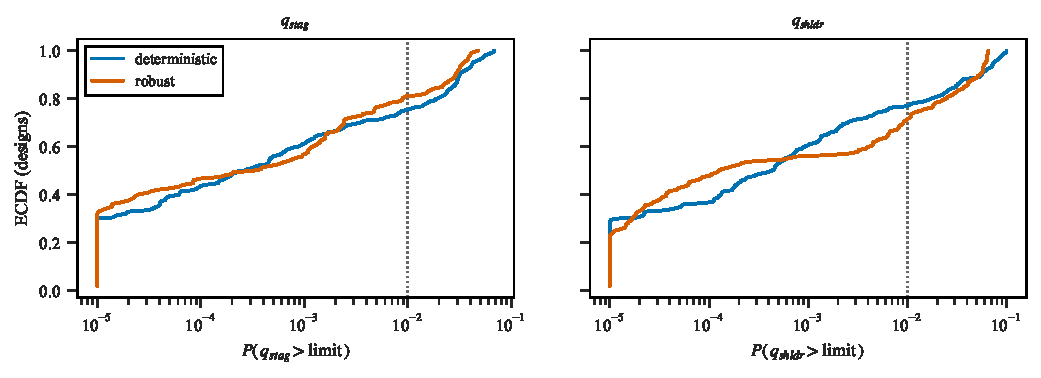
\includegraphics[width=\linewidth]{fig3_violation_ecdf}
\caption{Exceedance probabilities over each front. The deterministic
  front reaches $P(q_{\mathrm{stag}}>\mathrm{lim})=6.8\%$ and
  $P(q_{\mathrm{shldr}}>\mathrm{lim})=10.0\%$ at its worst members; the
  robust front roughly halves both (4.8\% / 6.6\%).}
\label{fig:violation}
\end{figure}
\begin{table}[htbp]
\centering
\caption{Post-hoc fragility audit of the deterministic front (moments
  under the uncertainty model, $n_z=2000$).}
\label{tab:audit}
\begin{tabular}{lc}
\toprule
statistic & value \\
\midrule
$\sigma_{Q_s}$ median (CV median) & \SI{30.3}{\mega\joule\per\square\metre} (22.8\%) \\
$P(q_{\mathrm{stag}}>\mathrm{lim})>1\%$ & 25\% of designs (max 6.8\%) \\
$P(q_{\mathrm{shldr}}>\mathrm{lim})>1\%$ & 23.5\% of designs (max 10.0\%) \\
$P(n_{\max}>\mathrm{lim})>1\%$ & 0\% of designs \\
$P(\mathrm{slow})$ & 0.35--0.49 \\
robust-feasible fraction (E$+2\sigma$) & 92\% \\
\bottomrule
\end{tabular}
\end{table}

\subsection{Knee designs}
\label{sec:knees}

For a concrete comparison, the knee of each front was extracted with the
anchor-hyperplane criterion of Branke et al.\ \cite{branke2004knees}; the
robust front's anchor points are affinely dependent (one design anchors
both $\mathrm{E}[Q_s]$ and $\sigma_{Q_s}$), so a pseudo-weight criterion is
used there as the documented fallback. Table~\ref{tab:knees} lists both
knees, the robust design nearest the deterministic knee in the
$(\mathrm{E}[Q_s],\mathrm{E}[sg])$ plane, and simulator-truth nominal
values for each.

The two knees occupy different points of the trade. The robust knee is the
better vehicle by the nominal simulator as well: volumetric efficiency
0.857 against 0.745 and a nominal range of 11{,}321 against 7{,}465~km,
paid for with a higher nominal heat load (183.9 vs
\SI{128.8}{\mega\joule\per\square\metre}). The matched comparison is more
sobering and more instructive: the robust design closest to the
deterministic knee in expected performance cuts $\sigma_{Q_s}$ by only
3.7\%, because the deterministic knee already sits near the dispersion
floor. The matched-pair advantage of Fig.~\ref{fig:matched} lives
overwhelmingly in the higher-performance region of the front, where heat
load and range are pushed toward their limits and dispersion grows; at the
low-load corner, both formulations converge on the same near-floor designs.
The slow-family probability separates the knees sharply (19\% against 48\%):
the robust knee buys its range partly through lofted, dispersed
trajectories, a trade the deterministic formulation cannot even express.

\begin{table}[htbp]
\centering
\caption{Knee-point designs of each front and the robust design nearest
  the deterministic knee in the $(\mathrm{E}[Q_s],\mathrm{E}[sg])$ plane;
  robust lens ($n_z=2000$), nominal values from the simulator at
  $\mathbf{z}_0$.}
\label{tab:knees}
\begin{tabular}{lccc}
\toprule
quantity & det knee & robust knee & robust matched \\
\midrule
$R_n$ [m]                  & 5.60  & 4.84  & 5.20 \\
$R_s$ [m]                  & 0.020 & 0.022 & 0.021 \\
$\theta_c$ [deg]           & 37.0  & 21.6  & 40.9 \\
$\eta_V$ [-]               & 0.745 & 0.857 & 0.725 \\
$Q_s$ at $\mathbf{z}_0$ (sim) [\si{\mega\joule\per\square\metre}]
                           & 128.8 & 183.9 & 119.8 \\
$sg$ at $\mathbf{z}_0$ (sim) [km]
                           & 7{,}465 & 11{,}321 & 6{,}514 \\
$\mathrm{E}[Q_s]$ [\si{\mega\joule\per\square\metre}]
                           & 117.4 & 164.1 & 110.6 \\
$\sigma_{Q_s}$ [\si{\mega\joule\per\square\metre}]
                           & 24.8  & 37.3  & 23.9 \\
$\mathrm{E}[sg]$ [km]      & 5{,}887 & 5{,}586 & 5{,}766 \\
$P(q_{\mathrm{shldr}}>\mathrm{lim})$ [\%]
                           & 0.01  & 0.32  & 0.004 \\
$P(\mathrm{slow})$ [\%]    & 19.4  & 48.0  & 43.3 \\
\bottomrule
\end{tabular}
\end{table}

\begin{figure}[htbp]
\centering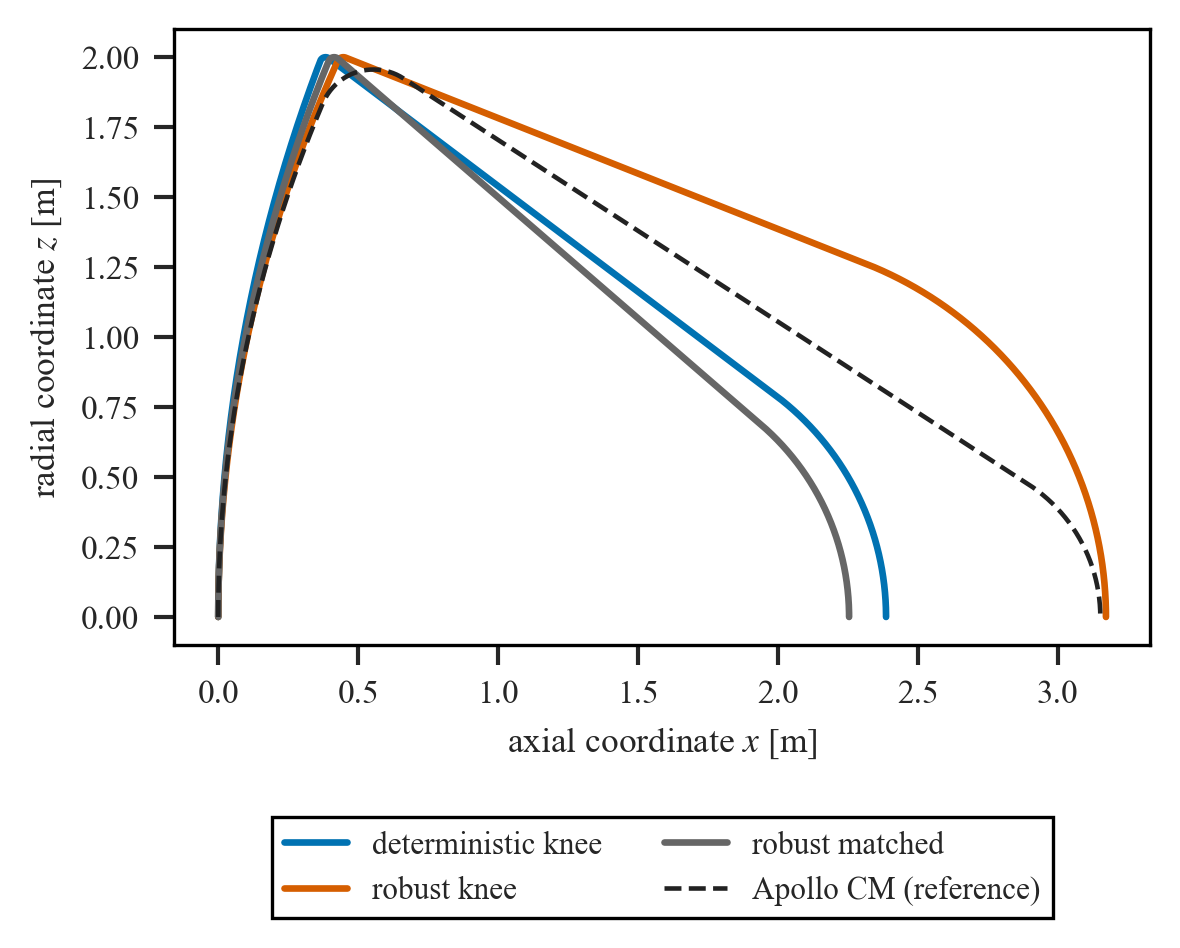
\includegraphics[width=0.8\linewidth]{fig7_silhouettes_knees}
\caption{Meridional outlines of the knee designs and the robust matched
  design of Table~\ref{tab:knees}, with the Apollo command module
  (dashed; drawn at its own body radius of \SI{1.956}{\metre}) for scale.
  The robust knee is the blunter, lower-cone shape
  ($R_n=\SI{4.84}{\metre}$, $\theta_c=21.6^\circ$); the deterministic
  knee and the matched design sit close together
  ($R_n\approx\SI{5.2}{\metre}$--$5.6$, $\theta_c=37$--$41^\circ$).}
\label{fig:silhouettes}
\end{figure}

\subsection{Design-space view}
\label{sec:designspace}

Figure~\ref{fig:designspace} maps the inflated $\sigma_{Q_s}$ over the
design space (300-point scan, $r_s$ slice) with both fronts overlaid. Both
formulations settle in the low-dispersion region of the space --- the
deterministic one by constructive accident, since low heat load and low
dispersion correlate through the same shallow-entry physics --- and the
floor binds everywhere on the map's cold side. The same scan confirms the
$P(\mathrm{slow})$ finding of Section~\ref{sec:robform}: family
probability varies only between 0.34 and 0.59 across the entire space.
Geometry does not buy direct descent under a $\pm0.5^\circ$
flight-path-angle dispersion; corridor and guidance levers would have to.

\begin{figure}[htbp]
\centering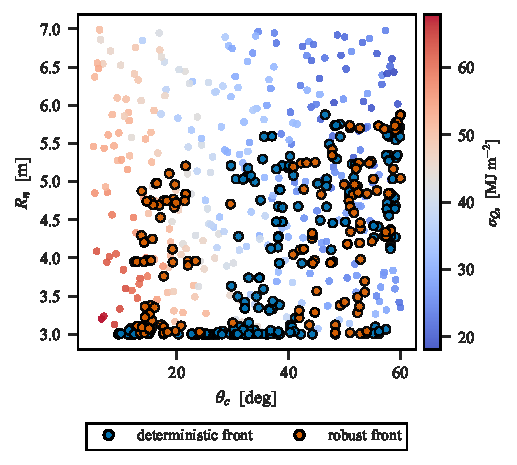
\includegraphics[width=\linewidth]{fig5_design_space_sigma_map}
\caption{Inflated $\sigma_{Q_s}$ over the design space (300-point scan,
  $r_s$ slice) with both fronts. Both fronts hug the low-dispersion
  region; the floor binds everywhere.}
\label{fig:designspace}
\end{figure}

\subsection{Deterministic exploitation of surrogate epistemics}
\label{sec:exploit}

The audit surfaced one more consequence of point-prediction optimization,
this one methodological. Fifty-four of the 200 deterministic designs carry
a surrogate range prediction at $\mathbf{z}_0$ above
\SI{20015}{\kilo\metre} --- above the antipodal great-circle distance, the
physical maximum of the quantity being optimized. The mechanism is the
slow-family range GP: in the deterministic problem, $sg(\mathbf{z}_0)$ is a
plain mixture prediction, and in the lofted corner the slow-GP mean
extrapolates far outside its training support (at the deterministic knee
the slow-GP mean is $10^5$~km). The optimizer, maximizing range, walked
straight into that blind spot: the surrogate claims
$\SI{26004}{\kilo\metre}$ at the deterministic knee where the simulator
returns \SI{7465}{\kilo\metre} --- a factor of 3.5. The robust formulation
does not fall into the same trap, for a structural reason:
$\mathrm{E}[sg]$ is formed by averaging the mixture over the uncertainty
sample, which damps any single extrapolating component, and the resulting
robust front spans $\mathrm{E}[sg]=4{,}117$--$6{,}393$~km, entirely within
the physical envelope. The lesson generalizes: a probabilistic surrogate
optimized through its point predictions will be exploited wherever its
mean leaves the data, and moment objectives --- or any formulation that
averages over the uncertainty space --- self-regulate against exactly this
failure. All nominal-range values quoted in this paper for specific
designs (Table~\ref{tab:knees} and Section~\ref{sec:verification}) come
from the simulator, never from the surrogate at $\mathbf{z}_0$.

\subsection{Sensitivity of the comparison to the uncertainty model and
matching construction}
\label{sec:sens}

The comparison rests on one uncertainty model and one matching window, so
both were stress-tested. Each front was re-evaluated through the same
common-random-number moment engine under five alternative uncertainty
models --- the aerodynamic band widened and narrowed
($\sigma_k=0.03,\,0.07$), the two scale factors correlated
($\rho=0.8$, addressing the weakest assumption of
Section~\ref{sec:uncertainty}), and the flight-path-angle dispersion
halved and enlarged by half ($\sigma_{\gamma_0}=0.25^\circ,\,0.75^\circ$)
--- using the same Latin-hypercube seed, with shared $\gamma_0$/$V_0$
quantiles wherever the distributions allow. The baseline configuration
reproduces the statistics of Tables~\ref{tab:matched} and \ref{tab:audit}
exactly, anchoring the comparison. Table~\ref{tab:sens} reports the
resulting statistics.

\begin{table}[htbp]
\centering
\caption{Sensitivity of the comparison statistics to the uncertainty
  model (both fronts re-evaluated through the same moment engine,
  $n_z=2000$; baseline column reproduces Tables~\ref{tab:matched} and
  \ref{tab:audit}).}
\label{tab:sens}
\begin{tabular}{lcccccc}
\toprule
statistic & base & $\sigma_k{=}0.03$ & $\sigma_k{=}0.07$ &
$\rho{=}0.8$ & $\sigma_{\gamma_0}{=}0.25^\circ$ &
$\sigma_{\gamma_0}{=}0.75^\circ$ \\
\midrule
$\sigma_{Q_s}$ floor, robust front [MJ/m$^2$]
  & 16.4 & 16.0 & 16.8 & 16.2 & 13.0 & 20.5 \\
det.-front $\sigma_{Q_s}$ median [MJ/m$^2$]
  & 30.3 & 29.9 & 30.8 & 30.1 & 24.1 & 37.4 \\
det.-front max $P(q_{\mathrm{shldr}}>\mathrm{lim})$ [\%]
  & 10.0 & 10.0 & 9.9 & 9.9 & 1.5 & 17.8 \\
det.\ designs with a match
  & 196 & 195 & 197 & 195 & 195 & 188 \\
matched pairs
  & 5{,}371 & 5{,}316 & 5{,}418 & 5{,}238 & 7{,}398 & 3{,}719 \\
pairs favouring robust [\%]
  & 98.1 & 98.1 & 98.0 & 98.0 & 98.6 & 96.3 \\
pair-level median $\sigma$ cut [\%]
  & 27.5 & 27.6 & 27.2 & 27.0 & 36.6 & 17.2 \\
design-level median $\sigma$ cut [\%]
  & 35.0 & 35.4 & 34.4 & 35.2 & 43.0 & 33.8 \\
\bottomrule
\end{tabular}
\end{table}

Three observations. First, the comparison is indifferent to the
aerodynamic model-form specification: across $\pm40\%$ of the scale band
and a strongly correlated pair, every statistic moves within a percentage
point, and the dispersion floor stays between 16.0 and
\SI{16.8}{\mega\joule\per\square\metre}. The floor is not an artefact of
the aerodynamic uncertainty --- which is exactly what
Section~\ref{sec:fronts} claims. Second, the entry-state dispersion moves
the absolute levels as it must (the floor scales with
$\sigma_{\gamma_0}$: 13.0, 16.4, \SI{20.5}{\mega\joule\per\square\metre}
at 0.25, 0.5, 0.75$^\circ$; the hidden worst-case exceedance probability
scales from 1.5\% to 17.8\%; robust-style feasibility of the deterministic
front from 100\% down to 78.5\%), but the comparison conclusions do not:
across a factor-three range of $\sigma_{\gamma_0}$, the fraction of pairs
favouring the robust front stays between 96.3 and 98.6\%, and the
design-level median cut between 33.8 and 43.0\%. The fragility finding is
a faithful image of the dispersion it reflects, not of one chosen band.
Third, the matching construction is not doing the work: with the window
widened from $\pm1\%$ to $\pm5\%$, the pair count grows from 4{,}766 to
7{,}136 while the fraction favouring robust moves only from 99.1\% to
94.4\%, the pair-level median cut stays within $27.5\pm1$ percentage
points, and the design-level median cut within $35.9\pm1.5$. A further
variation addresses the range leg specifically, because that leg carries
the surrogate's $\mathrm{E}[sg]$ bias (Section~\ref{sec:verification}):
holding the heat-load leg at $+2\%$ and widening only the range leg ---
to 5, 10, 15\%, and complete removal --- moves the pair preference from
98.1\% to no less than 97.2\% and the pair-level median cut from 27.5\%
to 32.2\%, the cuts growing because lower-range robust designs disperse
less. No differential bias of the surrogate's range prediction can
therefore overturn the comparison through the matching construction.
Finally, the
headline statistics are stable across optimizer seeds: three independent
robust runs give matched-pair preferences of 97.4--98.1\%, design-level
median cuts of 31.9--35.0\%, and the same dispersion floor to three
significant figures (16.36--\SI{16.4}{\mega\joule\per\square\metre};
Appendix~\ref{app:seeds}); the nearest-match statistic is the most
seed-sensitive (designs improved 68.9--84.2\%) but its conclusion holds
on every seed.
